\documentclass[11pt, solution, letterpaper]{format}
\usepackage[utf8]{inputenc}
\setlength{\parindent}{0 in}

\usepackage{amsmath}
\usepackage{graphicx}
\graphicspath{ {./images/} }
\usepackage[utf8]{inputenc}
\usepackage{enumerate}
\usepackage{amsmath,amssymb,amsthm}
\usepackage{listings}
\renewcommand{\qedsymbol}{$\blacksquare$}
\setlength\parindent{0pt}
\usepackage{tikz}
\usepackage{pgf}
\usepackage{tikz}
\usetikzlibrary{arrows,automata}
\usepackage{hyperref}
\newcommand{\noin}{\noindent}
\usepackage{enumerate}
\usepackage{tikz}
\usepackage{pgf}
\usepackage{tikz}
\usepackage{hyperref}
% \usepackage{booktabs}
\usepackage{cancel}

% \pagestyle{empty}

\setlength{\oddsidemargin}{-0.25 in}
\setlength{\evensidemargin}{-0.25 in}
\setlength{\topmargin}{-0.9 in}
\setlength{\textwidth}{7.0 in}
\setlength{\textheight}{9.0 in}
\setlength{\headsep}{0.75 in}
\setlength{\parindent}{0 in}
% \setlength{\parskip}{-.10 in}
\usepackage{epsf}
\usepackage{pseudocode}
% \usepackage{times}
% \usepackage{mathptm}

\def\O{\mathop{\smash{O}}\nolimits}
\def\o{\mathop{\smash{o}}\nolimits}
\newcommand{\e}{{\rm e}}
\newcommand{\R}{{\bf R}}
\newcommand{\Z}{{\bf Z}}
\newcommand\tab[1][1cm]{\hspace*{#1}}




\begin{document}
Problem Set 5\\
Julia Pearl\\

I collaborated with Rodrigo Daboin Sanchez and Noah Epstein. All code and problems were done independently.
\clearpage
\section{Birthdays and Hashes}
Suppose each person gets a random hash value from the range [1...n]. (For the case of birthdays, n would be
365.) Show that for some constant $c_1$, when there are at least $c_1*\sqrt{n}$ people in a room, the probability that no two have the same hash value is at most $\frac{1}{e}$. Similarly, show that for some constant $c_2$ (and sufficiently large n), when there are at most $c_1*\sqrt{n}$
people in the room, the probability that no two have the same hash value is at least $\frac{1}{2}$. Make these constants as close to optimal as possible.\\ Hint: you may use the fact that
$e^{-x} \geq 1 - x $\\ and\\ $e^{- x - x^2} \leq 1-x$ for $x \leq \frac{1}{2}$.\\ You may feel free to find and use better bounds.

a. We will first find the probability that no two people have the same hash value. This is very similar to the probability that no two people have the same birthday, except instead of 365, we use the term n.

For initial clarity's sake, in we can say that $x = c_1\sqrt{n}$
\begin{equation*}
  \prod_{k=1}^{x - 1} (1 - \frac{k}{n})
\end{equation*}
We use the property $e^{-x} \geq 1 - x $, which is valid because we are finding an upper bound:
\begin{equation*}
  \prod_{k=1}^{x - 1} (1 - \frac{k}{n}) 
  \leq  \prod_{k=1}^{x - 1} e^{\frac{-k}{n}}
  = e^{\frac{\sum_{k=1}^{x - 1} -k}{n}}
  = e^{\frac{-x(x-1)}{2n}}
\end{equation*}

We are trying to find bounds for $c_1$ so that the probability of no two people having the same hash value, $e^{\frac{-x(x-1)}{2n}}$, is at most (or less than or equal to) $\frac{1}{e}$.

\begin{equation*}
  e^{\frac{-x(x-1)}{2n}}
  \leq  \frac{1}{e}
  = e^{-1}
\end{equation*}
Because the bases are the same, positive value, we can compare the exponents:
\begin{equation*}
  \frac{-x(x-1)}{2n}
  \leq -1
\end{equation*}
Replacing $c_1\sqrt{n}$ for x:
\begin{equation*}
  \frac{-c_1\sqrt{n}(c_1\sqrt{n} - 1)}{2n}
  \leq -1
\end{equation*}
\begin{equation*}
  \frac{-c_1(c_1\sqrt{n} - 1)}{2\sqrt{n}}
  \leq -1
\end{equation*}
\begin{equation*}
  c_1^2\sqrt{n} - c_1)
  \geq 2\sqrt{n}
\end{equation*}
\begin{equation*}
  c_1^2\sqrt{n} - 2\sqrt{n})
  \geq c_1
\end{equation*}
\begin{equation*}
  \sqrt{n}(c_1^2 - 2)
  \geq c_1
\end{equation*}
Now, we know that n is reasonably large. Thus, as long as $(c_1^2 - 2) > 0$, this must be a valid equation. Because the number of people must be positive, we can focus on the positive root of this equation $\sqrt{2}$. \\We are left with the lower bound of $\sqrt{2}$. \\
\clearpage
b. Now, we will focus on showing that the probability that no two people have the same hash value is greater than or equal to $\frac{1}{2}$. \\
We can set the probability of no two people sharing a hash just like we did in the first part of the problem, except $x = c_2\sqrt{n}$
\begin{equation*}
  \prod_{k=1}^{x - 1} (1 - \frac{k}{n}) 
  \leq  \prod_{k=1}^{x - 1} e^{\frac{-k}{n}}
  = e^{\frac{\sum_{k=1}^{x - 1} -k}{n}}
  = e^{\frac{-x(x-1)}{2n}}
\end{equation*}
Now, we set this probability to be greater than or equal to $\frac{1}{2}$ or $e^{-ln2}$.

\begin{equation*}
  e^{\frac{-x(x-1)}{2n}}
  \geq e^{-ln2}
\end{equation*}
Because the bases are the same, positive value, we can compare the exponents:
\begin{equation*}
  \frac{-x(x-1)}{2n}
  \leq -ln2
\end{equation*}
Replacing $c_2\sqrt{n}$ for x:
\begin{equation*}
  \frac{-c_2\sqrt{n}(c_2\sqrt{n} - 1)}{2n}
  \geq -ln2
\end{equation*}
\begin{equation*}
  \frac{c_2(c_2\sqrt{n} - 1)}{2\sqrt{n}}
  \leq ln2
\end{equation*}
\begin{equation*}
  c_2(c_2\sqrt{n} - 1)
  \leq 2ln2\sqrt{n}
\end{equation*}
\begin{equation*}
  c_2(c_2\sqrt{n} - 1)
  \leq 2ln2\sqrt{n}
\end{equation*}
\begin{equation*}
  \sqrt{n}(c_2^2 - 2ln2)
  \leq c_2
\end{equation*}
The left side of this equation holds n and $c_2^2$. We know that n is reasonably large, and we know that $c_2^2$ is larger than $c_2$. For the left side to be smaller than the right side, $(c_2^2 - 2ln2)$ must be less than or equal to 0. We can set up and solve this equation, ultimately finding the correct bounds of $c_2$. 
\begin{equation*}
  (c_2^2 - 2ln2)
  \leq 0
\end{equation*}
\begin{equation*}
  c_2^2 
  \leq 2ln2
\end{equation*}
\begin{equation*}
  -\sqrt{2ln2} \leq
  c_2 
  \leq \sqrt{2ln2}
\end{equation*}
These are the bound of $c_2$ that make the probability that two people do not share a hash value at least \frac{1}{2}.



\clearpage
\section{Bloom Filters}
A problem with Bloom filters is that you cannot delete elements from a Bloom filter by changing the corresponding 1s to 0s. (This was discussed in section.) Counting Bloom filters are a variation of Bloom filters
where you do not use an array of bits, but an array of small counters. Instead of changing 0s to 1s when an
element hashes to a Bloom filter location, you increment the counter. To delete an element, you decrement the
counter. To check if an element is in the set, you just check if all of the counter entries are bigger than 0; if
they are, then you return the element is in the set. If you see a 0, you say that the element is not in the set.\\
Deletions will work properly for a Counting Bloom filter as long as the counters never overflow; once a counter
overflows, you would not have an accurate count of the number of elements currently hashed to that location.
A standard choice in this setting in practice to use 4 bit counters. Find an expression for the probability that
a specific counter overflows for the cases of using 3 bit counters, 4 bit counters, and 5 bit counters when
n elements are hashed into m total locations using k hash functions. (You may have a summation in your
expression.) Calculate these probabilities when [k = (m/n)·ln 2], n = $10^5$, and m = $10^6$, reasonable numbers
for some practical situations. What sized counter do you think might be appropriate to use in practice?\\

\textbf{Application of a Bloom Filter}\\
For this problem, we will define the application of a bloom filter as running each of the n elements through each of the k filters and updating the corresponding counter of the m locations after every filter. Thus, we are really incrementing our counters a total of n*k times.\\

\textbf{Calculation of Overflow}\\
We can calculate the probability of an overflow using a binomial distribution. The probability of any element hashing to a specific location is $\frac{1}{m}$. The probability of an element not hashing to that location is $\frac{m - 1}{m}$.  When we calculate the probability of overflow of an array with b bits, we are calculating the probability that of our n*k elements, a number greater than or equal to $2^b$ elements will hash to a particular bin. This is enough information to create our binomial distribution:\\

$$\sum_{i=2^b}^{nk} {nk \choose i}*(\frac{1}{m})^i*(\frac{m-1}{m})^{nk-i}$$

This is the same as calculating the 1 minus the probability that of our n*k elements, a number less than $2^b$ elements will hash to a particular bin.  However, Wolfram mathematica (for some reason) was able to calculate this term above rather than the term:
$$1 - \sum_{i=1}^{2^b} {nk \choose i}*(\frac{1}{m})^i*(\frac{m-1}{m})^{nk-i}$$

I tried to reformat the above term into:
$$1 - \sum_{i=1}^{2^b} \frac{1}{i!} * (\prod_{j = 0}^{i - 1} \frac{nk - j}{m})*(\frac{m-1}{m})^{nk-i}$$

But worlfram alpha was not able to calculate that either.\\

For 3 bits, 4 bits, and 5 bits, the following answers were calculated when plugging in k = (m/n)·ln 2, n = $10^5$, m = $10^6$, and b = number of bits (3, 4, or 5): \\
3 bits: $7.15404*10^{-7}$\\
4 bits: $7.07171 * 10^{-17}$\\
5 bits: $1.56361 * 10^{-41}$\\

All three of these numbers are pretty small probabilities of overflow. If there is a case in which very terrible things (or just high risk events) would happen in the event of an overflow, perhaps 4 or 5 bits might be safest. If space is an issue, then the 3 bit overflow probability is low enough that 3 bits could be used. 

\clearpage
\section{Super Sketchy Document Similarity}
For the document similarity scheme described in class, it would be better to store fewer bytes per document.
Here is one way to do this, that uses just 48 bytes per document: take an original sketch of a document, using
84 different permutations. Divide the 84 permutations into 6 groups of 14. Re-hash each group of 14 values to
get 6 new 64 bit values. Call this the super-sketch. Note that for each of the 6 values in the super-sketch, two
documents will agree on a value when they agree on all 14 of the corresponding values in the sketch. Why
does it make sense to simply assume that this is the only time a match will occur?\\

Consider the probability that two documents with resemblance r agree on two or more of the six sketches.
Write equations that give this probability and graph the probability as a function of r. Explain and discuss
your results.\\

What happens if instead of using a 64 bit hash value for each group in the supersketch, we only use a 16 bit
hash? An 8 bit hash?\\

\textbf{Probability of Matching Hashes}
The probability that hash values will match (after the super-sketch) is equal to the probability of an actual match of values (resemblance r), plus the probability of not a match but a collision.\\

In the case of 64 bits, the sum of these two probabilities is:\\
$$m = r + \frac{(1 - r)}{2^{64}}$$

\textbf{A Negligible Collision}\\
Because resemblance r is greater than or equal to 0, the largest that the second term of m can be is equal to $2^{-64}$, or $5.42 * 10^{-20}$.  Because this is such a small number in general and in relation to r (which without more document information we can assume to be a uniform value in the range [0, 1]), this is a negligible  term. Thus, when considering the probability of an actual match in the case of 64 bits, it makes sense to assume that the probability of values matching is equal to only the first term, the probability of an actual match. \\

\textbf{Graphing m vs. r}\\
Because of the question of changing bit values, even though the second term of m is negligible for 64 bits, as we calculate and graph the probabilities of at least two sketch agreements, we will continue to graph using the m term. When we consider 16 and 8 bit hashes, we will change the value of m and note the potential differences in graphs. We know at the very least that for 64 bits, the collision term does not impact the graph.\\

\textbf{Probability of Full Super-Sketch Agreement}\\
The probability that two sketches agree is $m^{14}$. The probability that two sketches do not agree is $(1 - m^{14})$.\\


\textbf{Probability of at least 2 Full Super-Sketch Agreement}\\
We can calculate the probability that a specific number of full super-sketches do agree out of the six total using the binomial function. Instead of calculating the probability of at least 2, we can calculate 1 minus the probability that no sketches agree minus the probability that only one sketch agrees. For our binomial, p = $m^{14}$, m = 6, and k will equal 0 and then 1.  Thus, the probability that at least two full sketches agreeing is the following:\\
$$\text{1 - P(no sketches agree) - P(1 sketch agrees)}$$
$$ = 1 - (1 - m^{14})^6 - {6 \choose 1}(m^{14})^1(1 - m^{14})^5 $$

\textbf{Graphing the 64 bit hash}\\
Graphing this probability for a 64 bit hash as a function of m yields the following image:\\
\begin{center}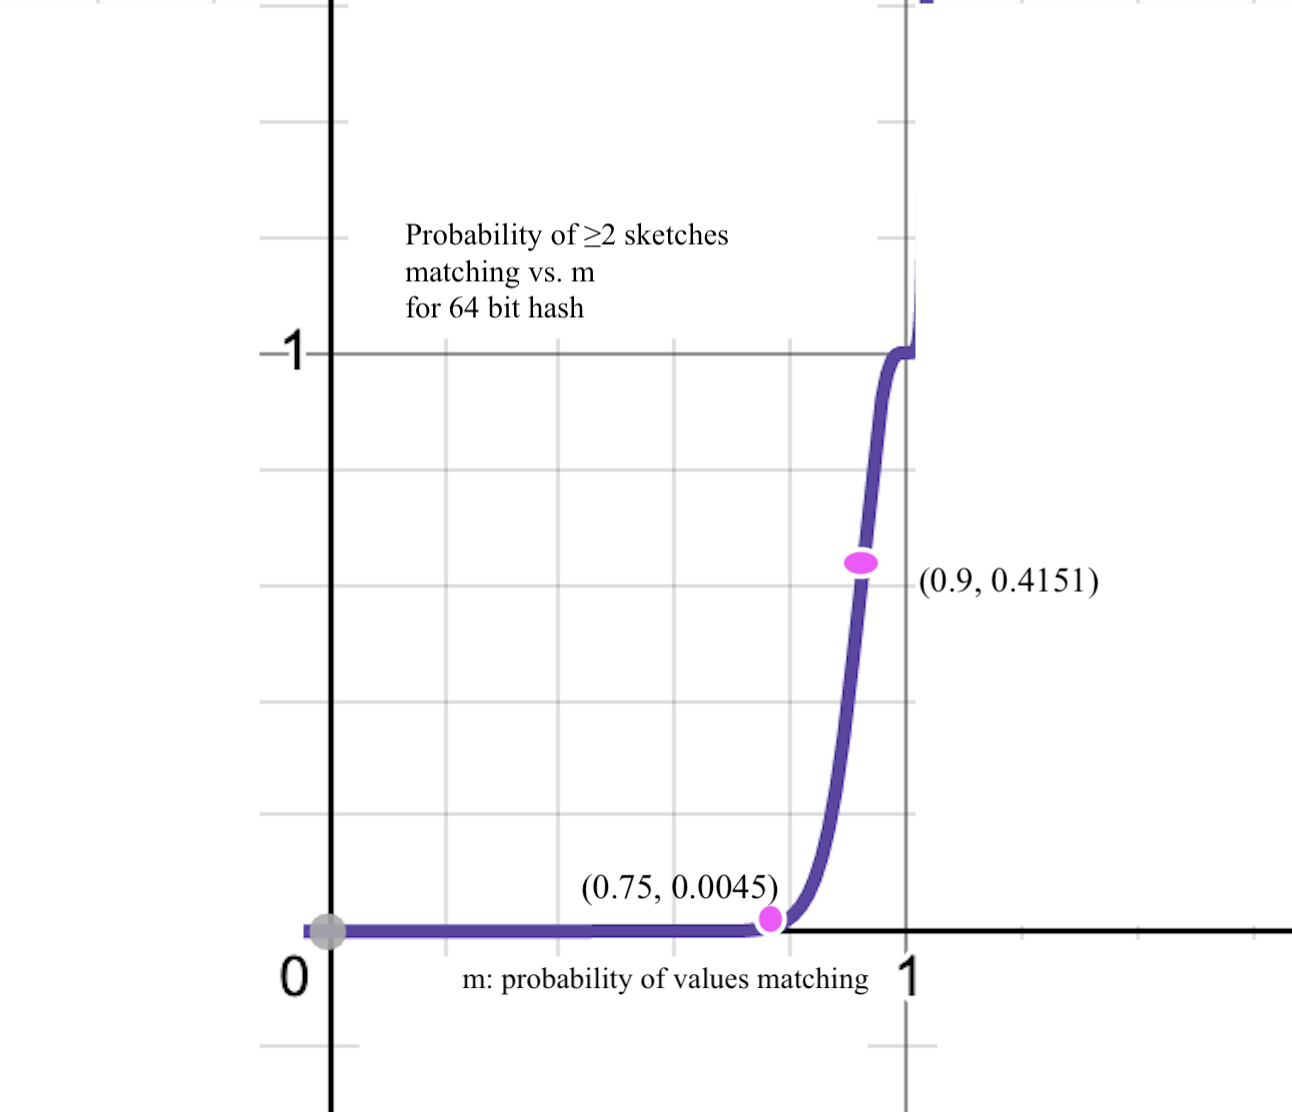
\includegraphics[scale=.5]{64bit.png}]\end{center}

Reiterating, m is equal to the probability of 2 sketches matching (via individual, in-array matches or in-array collisions). 
We can see that m is close to 0 until the resemblance reaches 0.75. Then, as resemblance transitions to 0.9, the probability of at least 2 sketches matching is equal to 0.42. Finally, when the probability of resemblance is equal to 1, the probability of at least 2 matches reaches 1 as well. As r increases, the amount of collisions decrease (because collisions are based upon a match not occurring). Because resonance is very much the dominating term of m, as  r increases, m increases (or m is proportional to r). This graph shows that once the documents have a resemblance of 75 percent, from there, the likelihood that 2 or more sketches will match grow very quickly. \\

\textbf{Graphing the 16 bit hash}\\
Below is the graph of m when the hash is a 16 bit hash.\\
\begin{center}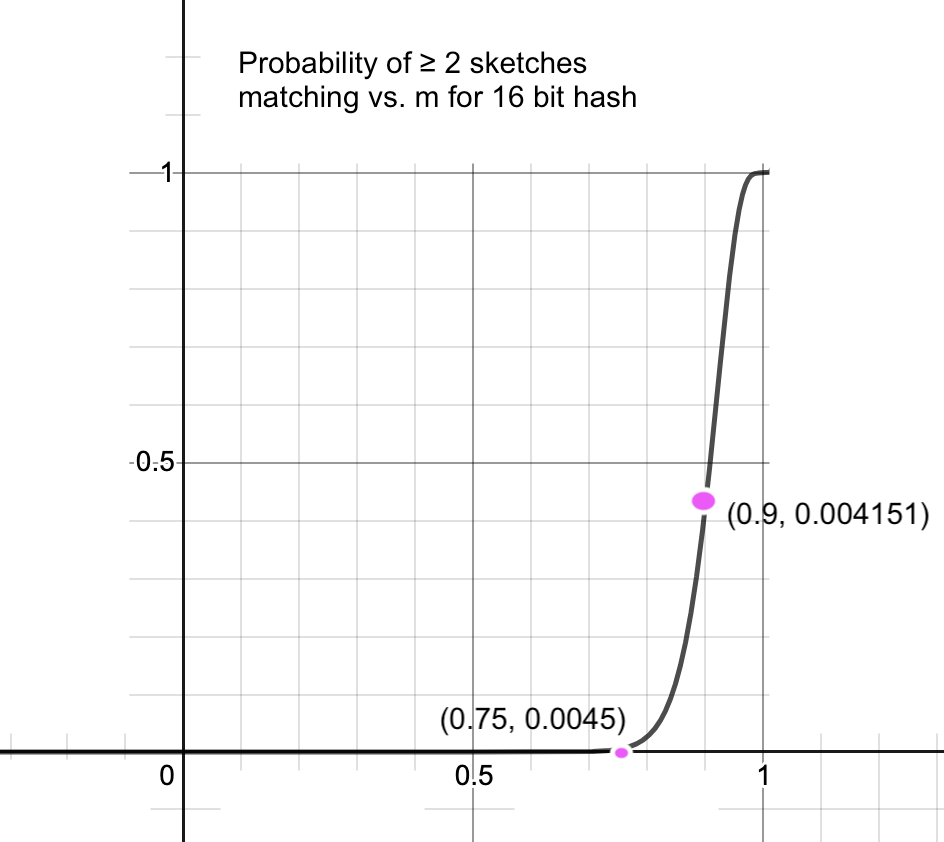
\includegraphics[scale=.5]{16bit.png}\end{center}

This graph is very similar to the 64 bit hash. The points on the graph to the precision of 4 decimal points are equal in the 16 bit to the 64 bit. \\
\begin{center}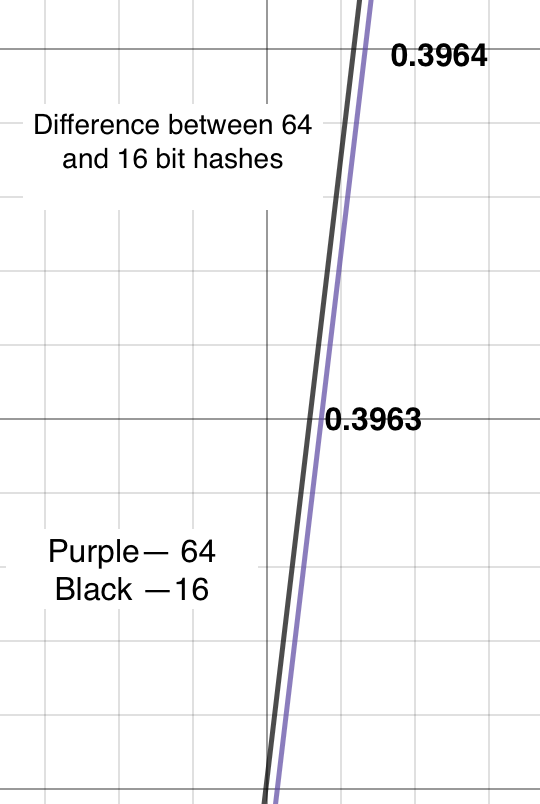
\includegraphics[scale=.5]{16-64.png}\end{center}

Zooming in to the precision of 4 decimal points on the graph of the 64 bit and the 16 bit, there is a very small difference in the graphs. We can say that the difference between a 64 bit hash and a 16 bit hash is minimal.

\textbf{Graphing the 8 bit hash}\\
Below is the graph of m when the hash is an 8 bit hash.\\
\begin{center}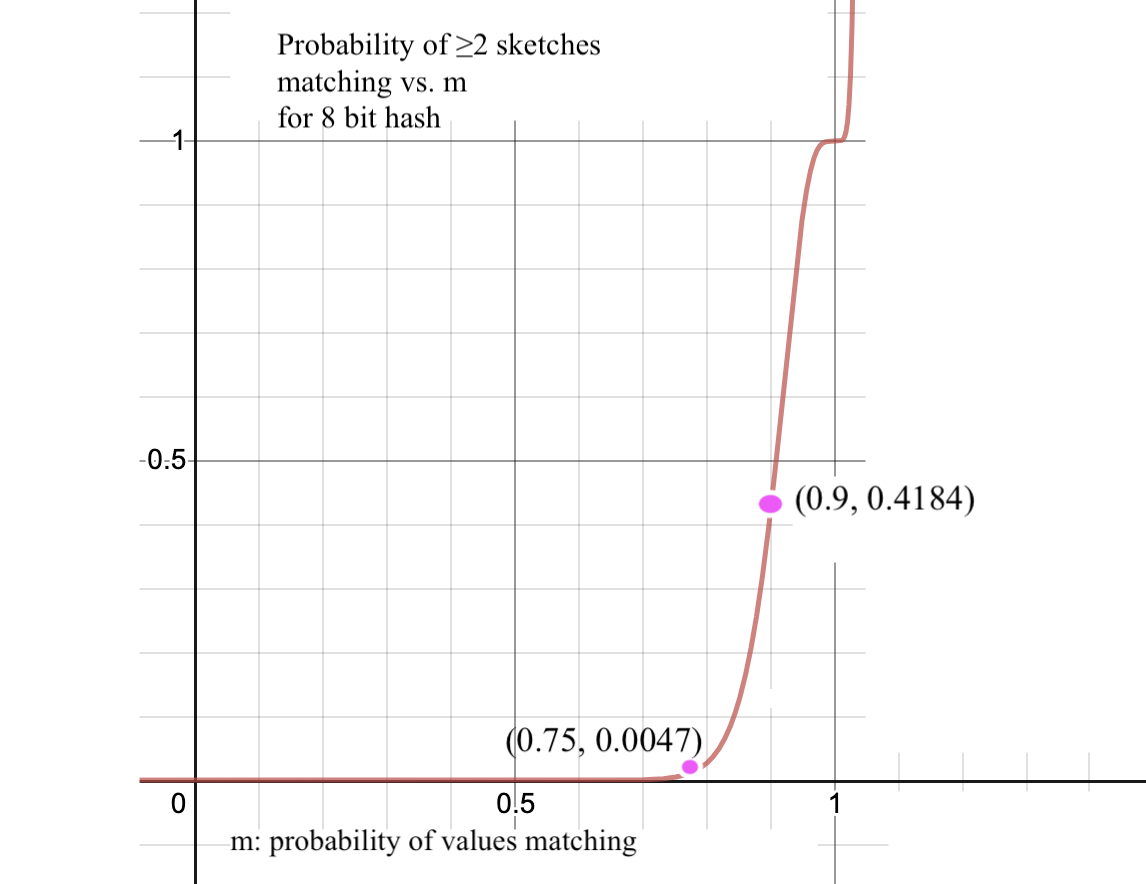
\includegraphics[scale=.5]{8bit.png}\end{center}

This graph is similar to the 64 bit hash. The points on the graph to the precision of 3 decimal points differ slightly. \\
\begin{center}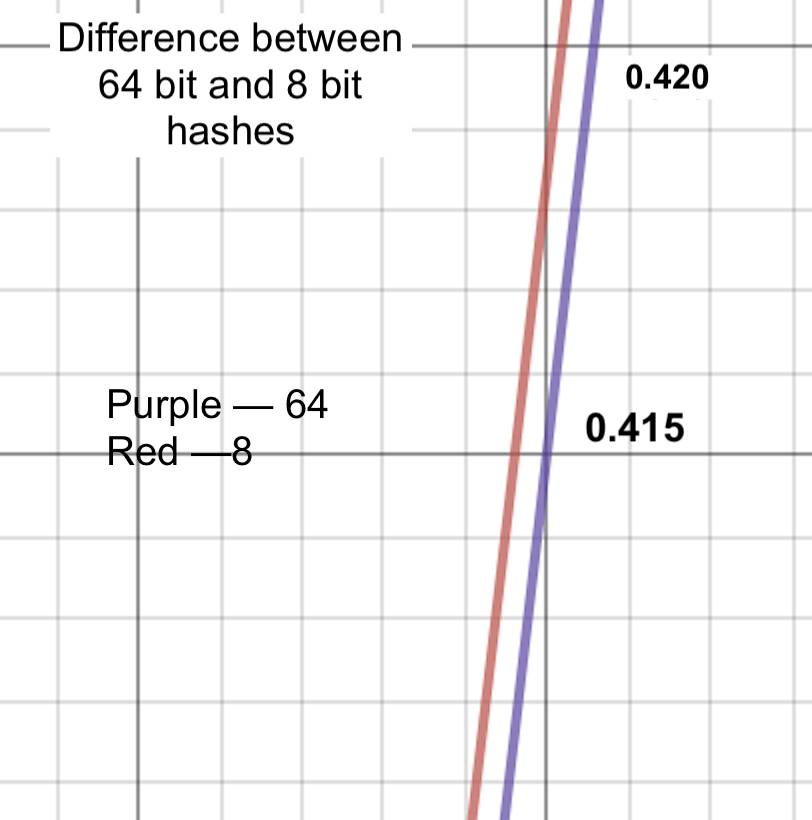
\includegraphics[scale=.5]{8-64bit.png}\end{center}

Zooming in to the precision of 2 decimal points on the graph of the 64 bit and the 8 bit, there is a notable but still small difference in the graphs. We can say that the difference between a 64 bit hash and a 8 bit hash is moderately minimal. If the size of the documents were very large, then this difference may be problematic.
\clearpage
\section{Multi-Part: Appropriate Witness $\&$ RSA Encryption}
Prove that 636127 is composite by finding an appropriate witness. Be sure to give ample evidence showing that your witness is in fact witnesses. (Note: do not use a factor as a witness! Sure, these numbers are small enough that you can exhaustively find a factor; that is not the point. A factor is not a 1 witness, according to our definition.) Hint: you will want to write some code. You will preferably use a
package that deals with big integers appropriately, as you may want to use some of this code for the next
problem (RSA). We don’t need a code listing for this problem– a short summary of the output should
suffice.\\

\textbf{Code Explanation:}\\
To solve this problem, I coded Rabin-Miller. The code is listed below part b. Because our witness has a range of 2 to 636126, and I wanted to walk through the example witness that I found, I coded mine to output the smallest witness with a squaring step that occurs less than 5 times. The smallest witness that proves that 636127 is composite in less than 5 steps is 4125.\\

Let's walk through Rabin-Miller and show that 636127 is a composite using the witness 4125.\\
Our prime candidate is 636127. 
$$636127 - 1 = 636126 = 2^1*318063$$
$$4125^318063 \text{ mod }  636127 = 472199$$
$$4125^(2*318063) \text{ mod }  636127 = 476323$$
$$4125^2*318063 \text{ mod }  636127 = 1$$

Because we have found a nontrivial square root to 1 mod 636127 of 476323, we have proven that 636127 is composite, and that 4125 is a witness.

b.
The number 294409 is a Carmichael number. Prove that it is composite by finding a witness. Briefly
explain why Fermat’s little theorem won’t help.\\

Fermat's little theorem has a series of numbers, called Carmichael numbers, which are "a-pseudoprime" for any choice of $a$ (or potential witness) relatively prime to n. Using Fermat's little theorem on these Carmichael numbers will yield false-composite-negatives. **Both Fermat's little theorem and the Rabin-Miller theorem only prove that numbers are not prime or that they are composite. Both do not guarantee prime-ness**\\

Because I coded 4a for Rabin-Miller, I ran the same code from my 4a on 4b. Just like 4a, my code outputs the smallest witness with a squaring step that occurs less than 5 times. The smallest witness that proves that 294409 is composite in less than 5 steps is 2.\\

Let's walk through Rabin-Miller and show that 294409 is a composite using the witness 2.\\
Our prime candidate is 294409. \\
$$294409 - 1 = 294408 = 2^3*36801$$
$$2^36801 \text{ mod } 294409 = 512$$
$$2^(2*36801) \text{ mod }  294409 = 262144$$
$$2^(4*36801) \text{ mod }  294409 = 1$$

Because we have found a nontrivial square root to 1 mod 294409 which is 262144, we have proven that 294409 is a composite, and that 2 is a witness.\\

The code for a and b is listed below:
\begin{lstlisting}
import java.math.BigInteger;
 

class rabmil {
    public static void main(final String[] args) {
        if (args.length != 1) {
            System.out.println("Please enter n");

        } else { 
            BigInteger n = new BigInteger(args[0]);
            BigInteger[] answer = new BigInteger[2];
            answer = M_finder(n.subtract(BigInteger.ONE), BigInteger.ZERO);
            System.out.println("M: " + answer[0] + "| K:  " + answer[1]);
            BigInteger a = BigInteger.valueOf(2);
            boolean witness = false;
            while ((witness == false) && (a.compareTo(n.subtract(BigInteger.ONE)) < 0)){                
                witness = RabbyTest(n, answer[0], a);
                a = a.add(BigInteger.ONE);
            }
            System.out.println(a.subtract(BigInteger.ONE));
        }
    }


    // returns [m, k]
    public static BigInteger[] M_finder (BigInteger n, BigInteger k){
        if (n.mod(BigInteger.valueOf(2)) == BigInteger.ZERO){
            n = n.divide(BigInteger.valueOf(2));
            k = k.add(BigInteger.ONE);
            return M_finder(n, k);
        } else {
            BigInteger[] answer = new BigInteger[]{n, k};
            return answer;
        }
    }
    
    public static boolean RabbyTest (BigInteger n, BigInteger m, BigInteger a){
        BigInteger b0 = a.modPow(m, n);
        if (b0.equals(BigInteger.ONE) || b0.equals(BigInteger.valueOf(-1))){
            return false;
        } else {  
            BigInteger i = RabbyLong(b0, n, 0);
            if (i.equals(BigInteger.ONE)){
                System.out.println("COMPOSITE!!! WITNES: " + a);
                return true;
            } else {
                return false;
            }
        }
    }

    public static BigInteger RabbyLong (BigInteger b, BigInteger n, int counter){
        if (counter == 5){
            return BigInteger.valueOf(-1);
        }
        b = b.modPow(BigInteger.valueOf(2), n);
        System.out.println("a^2(new m) mod n is " + b);
        if (b.equals(BigInteger.ONE) || b.equals(BigInteger.valueOf(-1))){
            return b;
        } else {
            return RabbyLong(b, n, counter + 1);
        }
    }
}
\end{lstlisting}
\clearpage
c. 
My RSA public key is: (46947848749720430529628739081,3726748626367923506206453697). Convert the message\\
$$\text{"Give me an A"}$$
into a number, using ASCII in the natural way. (So for “A b”: in ASCII, A = 65, space = 32, and b = 98;
translating each number into 8 bits gives “A b” = 010000010010000001100010 in binary.) Encode the
message as though you were sending it to me using my RSA key, and write for me the corresponding
encoded message in decimal.\\

I coded this in Java using the Big Integer class. First, I put n and e into Big Integers. My next step was turning the the string of "Give me an A" into a binary number. I went through the entire string left to right. I created an empty string binString to build the message's full binary term. For each letter, I converted it to a decimal ASCII number. Then, I converted the decimal number into binary. I checked the binary number and padded the left of the number when necessary to make sure the binary was a full 8 bits. I added each binary to the right side of binString. Then, I took binString and turned it into a Big Integer with base 10 (there is a building Big Integer property that allows a change of base given a string as an input). This yielded the message's decimal value in a Big Integer: 22100932013077800977026654273\\

Big Integer's have a modpow function, so I took the messgae's decimal valued Big Integer and took it to the e power (3726748626367923506206453697) and modded it by n (46947848749720430529628739081) to yield the final encrypted message:\\
27016764340118192395712492378\\

So, if I wanted to send the message "Give me an A" and my RSA public key was (46947848749720430529628739081, 3726748626367923506206453697), I'd send: \textbf{27016764340118192395712492378}\\

My code for this problem is written below:
\begin{lstlisting}
import java.math.BigInteger;

class rsa {
    public static void main(final String[] args) {            
        String m = "Give me an A";
        System.out.println(str_to_BigInt(m));
        BigInteger m_b = str_to_BigInt(m);
        BigInteger n = new BigInteger("46947848749720430529628739081");
        BigInteger e = new BigInteger("37267486263679235062064536973");
        m_b = m_b.modPow(e, n);
        System.out.println("Encryption: " + m_b);
    }

    public static BigInteger str_to_BigInt (String m){
        String build = "";
        for (int i = 0; i < m.length(); i++){
            int temp = (int)(m.charAt(i));
            String temp_str = Integer.toBinaryString(temp);

            while (temp_str.length() < 8){
                temp_str = "0" + temp_str;
            }
            build = build + temp_str;
        }
        BigInteger num = new BigInteger(build, 2);
        return num;
    }    
}
\end{lstlisting}

\clearpage
\section{1 Billion Balls}
(This problem worth 8 points) For the following problem you will write code to do some simulations. Suppose
I throw 1 billion balls into 1 billion bins (independently and uniformly at random). We will say for this experiment that the maximum load is the largest number of balls in any bin. Do this 100 times, and make a
table showing the frequency of the maximum load (that is, how many times the maximum load is x for any
relevant value of x).\\

Note: you do NOT want to create an array of 1 billion buckets, with the number of balls in each bucket. All
buckets with the same number of balls are indistinguishable in this experiment. So suppose you keep an array
A where A[i] is the number of bins with i balls. Can you do your simulation just keeping track of the A[i]?
(Trust me, this will be much easier.)\\

Now modify your experiment as follows. Suppose I throw 1 billion balls into 1 billion bins, sequentially,
the following way. When I throw a ball, I choose two bins independently and uniformly at random, and I put
the ball in the least loaded of the two bins. (That is, I put the ball in the bin with fewer balls, and break ties
whatever way you like.) Again, do this 100 times, and make a table showing the frequency of the maximum
load.\\

Write a few sentences describing your findings, and how you interpret them.\\

\textbf{The Problem}\\
I want my code to simulate throwing 1 billion balls into 1 billion bins. Then, I want my code to find the maximum number of balls that landed in the same bin for all of my billion bins. I cannot actually store 1 billion bins (1 billion sized array) and throw 1 billion balls (another billion of storage in the array) and then travel through my array and find a maximum of my billion throws (going through all of them is O(1 billion)). Storage and run time would be awful.\\

\textbf{The Array}\\
Instead, as the problem suggests, I have an array A in my code that, at each index i, stores the number of bins that contain i total balls. I coded this in Java, and the array is type Big Integers (which can handle values higher than 1 billion). Before any balls have been thrown, A has 1 billion bins - 1 at index 0.\\

\textbf{Randomly Generating a Number:}\\
I used Java's random number generator for the Big Integer class. I printed out the output for fifty trials, and it looked "fairly" random (or just had an okay spread).\\

\textbf{The Simulation}\\
The probability of throwing a ball into a bin that already contains i balls is equal to the number of bins that already have i balls (value stored in A[i]) plus 1 (because the values are 0 indexed) divided by the total number of bins (1 billion). 
$$ P(\text{Throwing a ball into a bin with max balls i}) = \frac{A[i] + 1}{1 \text{ billion}}$$
\textbf{Concept check:} this makes sense because at the beginning of the process, before we have thrown any balls, the probability that we throw our first ball into a bin that already contains 0 balls is 1. At any point when we are throwing balls into bins, all contents of bins stored in A will sum to 1 billion minus 1 (minus 1 because of the 0 index). \\


\textbf{Simulating Tossing Balls}\\
We can simulate the actual tossing of balls by generating a random number. We will generate a random number and judge, based upon the contents of A, the number of balls that were in the bin we have just "hit".  Once we know how many balls were in the bin we just hit, we can decrement and increment A appropriately: if we hit a bin previously containing m balls, now there is one less bin containing m balls and one more bin containing m + 1 balls. \\


Back to the generating of a number, we need to generate a number in the inclusive range of 0 to (1 billion - 1). Each A[i] contains the number of bins with total i balls. After we generate a random number, we go through A left to right to determine how many balls were in the bin we just hit. \\

We start at A[0]. Let's say that A[0] = j.  Thus, we can say that bins [0, j] have 0 balls. The probability of throwing a ball into one of these bins is j + 1/1 billion. When we generate a random number in the range of 0 to 1 billion - 1, the probability of generating a number less than or equal to j is j + 1/ 1 billion. So, if we generate a number in the range [0, j] or less than or equal to j, we just hit a previously empty bin! We can decrement A[0] and increment A[1]. \\

However, if we generate a number larger than j, we did not hit a bin in the [0, j] range. We then move on to A[1]. Let's say that A[1] contains the value k. We can say that bins [j + 1, j + k] contain 1 ball.  The probability of throwing a ball into a bin that already contains 1 ball is $\frac{k}{1 billion}$ (k + j - (j + 1) + 1). When we generate a random number in the range of 0 to 1 billion - 1, the probability of generating in the [j + 1, j + k] range is also $\frac{k}{1 billion}$. Because we know that the random number we have generated must be larger than j (because we have moved on to the first index), we can check to see if our random number is in the range only by comparing the random number to the max interval, or j + k. j + k represents the cumulative sum of A up to the index 1.  If the random number is less than or equal to j + k (again, the cumulative sum at A[1]), then we decrement A[1] and increment A[2]. However, if the random number is greater than the cumulative sum, the value must be in a range of [j + k + 1, 1 billion - 1], and we will proceed to check the rest of the array. The cumulative sum will eventually hit 1 billion - 1 because the sum of all values in array A is always equal to 1 billion - 1 (that's the maximum value of the random number generator, so we know that every value generated will have a correct placement spot in A).\\

\textbf{Maximum Number of Balls in One Bin}\\
The maximum number of balls in a single bin is equal to the size of array A.\\

\textbf{Cumulative Sum:}\\
At every point in the algorithm, [cumulative sum at A[i-1] + 1, cumulative sum at A[i]] represents the range of random number values that represent the probability of throwing a ball into a bin with max value i. This probability is the value stored in A[i] + 1 divided by 1 billion. The random number generator represents throwing a ball and hitting a bin with a max value of that specific range. The number of bins stored in A is always equal to the number of total bins.\\

\textbf{General Pattern in Psuedocode}\\
We can continue the simulation of throwing balls for every index in the steps written in psuedocode below:\\
1) Set a balls variable to 0. While balls is less than 1 billion, repeat the following steps:\\
2) Generate a random number r\\
3) Set a sum variable sum to equal 0\\
4) Set an increment variable i to equal 0\\
5) Add A[i] to sum.\\
6) If r is less than or equal to sum, decrement A[i] by 1 and increment A[i + 1] by 1. Break out of this loop.\\
7) If r is greater than sum, increment i by 1 and repeat steps  4-7.\\



\textbf{Space and Time Complexity:}\\
The worst case for space is O(n) in the $\frac{1}{10^81}$ probability that all balls land in the same bucket. The average maximum balls in one bin should be much much less than 1 billion (8 factors of 10 less). The upper bound for time is O($n^2$) also in the $\frac{1}{10^81}$ probability that all balls land in the same bucket. The lower bound for time is O(n) in the case that all balls land in different buckets (this is the probability of the birthday problem).\\

\textbf{Simulating Two Throws}\\
Because at each step, the random number is compared to a cumulative sum, a higher random number generated yields a higher bin placement. To simulate two throws, the code simply generates two numbers and picks the smaller number to place in a bin.\\

\textbf{Psuedocode for Two Throws}\\
The difference between this psuedocode and the psuedocode written for part 1 is stared**:\\
1) Set a balls variable to 0. While balls is less than 1 billion, repeat the following steps:\\
2) **Generate two random numbers. Pick the smaller one to be r.**\\
3) Set a sum variable sum to equal 0\\
4) Set an increment variable i to equal 0\\
5) Add A[i] to sum.\\
6) If r is less than or equal to sum, decrement A[i] by 1 and increment A[i + 1] by 1. Break out of this loop.\\
7) If r is greater than sum, increment i by 1 and repeat steps  4-7.\\

Results from Both Simulations\\
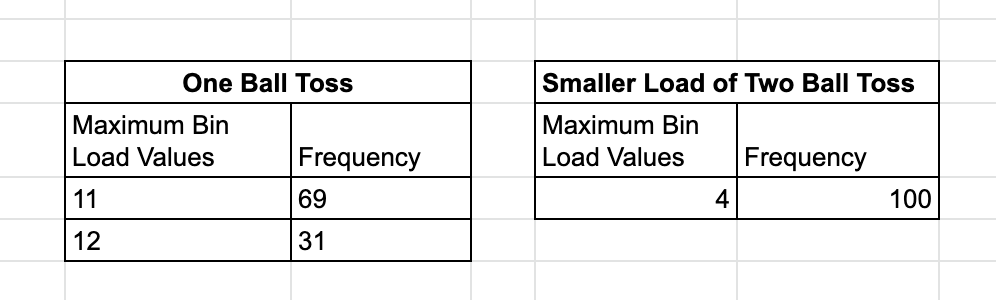
\includegraphics[scale=.75]{twoo.png}\\


\textbf{Comparisons}
The first part of the problem resulted in bins being filled with a maximum load of 11 and 12. 11 was more frequent than 12. Because such a large number of balls were thrown per trial, this explains the lack of variability in results (only producing two numbers). Also, 11 and 12 are numbers reasonably small enough to be a maximum load for 1 billion bins. \\

The second part of the problem results in bins being filled with a maximum load of 4 for every trial. Because an even larger number of balls were "thrown" per trial, the further lack of variability from part 1 is explained. Additionally, 4 is less than 11 and 12, which is as to be expected, and is moderately close to half of 11 and 12 (not that a factor of 2 is to be expected to appear in results, but proximity to a factor of 2 is affirming).\\

\textbf{Code:}\\
The code for problem 5 is written below:
\begin{lstlisting}
import java.math.BigInteger;
import java.util.Random;
import java.util.ArrayList;



class balls {
    public static void main(final String[] args) {
        if (args.length != 1) {
            System.out.println("Please indicate part 1 or 2");

        } else { 
            for (int i = 0; i < 46; i++){
                long startTime_2 = System.nanoTime();
                int top = fillBins(Integer.parseInt(args[0]));
                long endTime_2 = System.nanoTime();
                long duration = ((endTime_2 - startTime_2) / 1000000000);
                System.out.println(top);
            }
        }
    }

    public static int fillBins(int mode) {
        ArrayList<BigInteger> highs = new ArrayList<BigInteger>();
        BigInteger n = new BigInteger("999999999");
        highs.add(n);
        BigInteger i = BigInteger.ZERO;
        while(i.compareTo(n) <= 0){
            highs = throwABall(highs, mode);
            i = i.add(BigInteger.ONE);
        }   
        return (highs.size() - 1);
    }

    public static ArrayList<BigInteger> throwABall (ArrayList<BigInteger> highs, int mode){
        BigInteger d_rand = getRandomBigInteger(mode);
        int i = 0;
        BigInteger comp = BigInteger.ZERO;
        while (i < highs.size()){
            comp = comp.add(highs.get(i));
            if (d_rand.compareTo(comp) <= 0){
                int j = i + 1;
                comp.subtract(BigInteger.ONE);
                highs.set(i, (highs.get(i)).subtract(BigInteger.ONE));
                if (i == highs.size() - 1){
                    highs.add(BigInteger.ONE);
                } else {
                    highs.set(i + 1, (highs.get(i + 1)).add(BigInteger.ONE));
                }
                i = highs.size() + 1;
            } else {
                i++;
            }
        }
        return highs;
    }
 

    public static BigInteger getRandomBigInteger(int mode) {
        Random rand = new Random();
        BigInteger upperLimit = new BigInteger("999999999");
        BigInteger result_1;
        BigInteger result_2;
        do {
            result_1 = new BigInteger(upperLimit.bitLength(), rand); // (2^4-1) = 15 is the maximum value
        }while(result_1.compareTo(upperLimit) >= 0);   // exclusive of 13
        if (mode == 1){
            return result_1;
        }
        do {
            result_2 = new BigInteger(upperLimit.bitLength(), rand); // (2^4-1) = 15 is the maximum value
        }while(result_2.compareTo(upperLimit) >= 0); 
        return (result_1.min(result_2));
    }   
}
\end{lstlisting}

\end{document}